\documentclass[
11pt, paper=a4,  listof=totocnumbered, % lists are also included in table of contents
numbers=noendperiod, % Don't add a period at the end of a chapter number
]{scrreprt}

% ===============================
% IUBH Template für Seminar-, Bachelor-, and Master-works
% -------------------------------
% Authors; Ralf Kneuper, Jörg Sawatzki
% Maintainer: Paul Libbrecht

% Fix of Warning: Class scrreprt Warning: \float@addtolists detected!
% https://komascript.de/faq_float%40addtolist
\usepackage{scrhack}

% get custom bibliography style working without prepending [brackets]
\usepackage{natbib}
\setcitestyle{aysep={}} % remove comma as delimiter 

% breaks line at hyphens (resolves formatting issues in bibliography)
\usepackage[hyphens]{url}

\usepackage{txfonts} % Use a Times-new-roman open-source clone

\usepackage{caption}
\usepackage{float}

\setkomafont{chapter}{\Large} 
\setkomafont{section}{\large}
\setkomafont{subsection}{\large} 

\usepackage[left=2cm,right=2cm,top=2cm,bottom=2cm]{geometry} % margins
\addtolength{\footskip}{-0.7cm}% foot larger by 0,7 cm  (Raises the page number)


\usepackage[onehalfspacing]{setspace} % line space 1,5

\setlength{\parindent}{6pt} % Indent at start of paragraphs  6pt

\usepackage[utf8]{inputenc} %UTF-8 to encode many characters => for many characters, you can just input the character and avoid a macro

\usepackage[english]{babel} % english hyphenations
%\usepackage[T1]{fontenc} %wichtig für Trennung von Wörtern mit Umlauten
\usepackage{microtype} % align margins

\usepackage{graphicx} % import graphics
\usepackage{placeins}% places the graphics within text

% Abbreviation's directory
% printonlyused - only if used
% withpage - the first occurrence's page number is listed too
\usepackage[withpage]{acronym}

\usepackage[hidelinks]{hyperref} %https://tex.stackexchange.com/questions/823/remove-ugly-borders-around-clickable-cross-references-and-hyperlinks

\begin{document}

%TITELBLATT:!!!!!!!!!!!!!!!!!!!!!!!!!!!!!!!!!!!!!!!!!!!!!!!!!!!!!!!!!!!!!!!!!!!!!!!!!!!!!!!!!!!!!!!!!!!!!

\label{titlePage}
\begin{figure}[h]
\centering
\advance\leftskip--2cm

\includegraphics[width=0.75\textwidth]{pics/logo.pdf}
\end{figure}
\FloatBarrier

\begin{Large} 
\begin{center}
<Seminararbeit>
\end{center}
\end{Large} 

\vspace*{5mm}

\begin{large} 
\begin{center}
University of Applied Science - Online
\end{center}
\end{large} 

\begin{large} 
\begin{center}
Study-branch: Entomology
\end{center}
\end{large}

\vspace*{15mm}

\begin{Large} 
\begin{center}
\textbf{<Dies ist der Titel>}
\end{center}
\end{Large}

\vspace*{15mm}

\begin{large} 
\begin{center}
Maxi Musterfrau
\end{center}
\end{large} 

\vspace*{-6mm}

\begin{large} 
\begin{center}
Matrikelnummer: 010101001
\end{center}
\end{large} 

\vspace*{-6mm}

\begin{large} 
\begin{center}
Straße 10
\end{center}
\end{large} 

\vspace*{-6mm}

\begin{large} 
\begin{center}
realized in....
\end{center}
\end{large} 

\vspace*{5mm}

\begin{large} 
\begin{center}
Advisor: <Advisor>
\end{center}
\end{large} 

\begin{large} 
\begin{center}
Realized with input of the Parameter Generator: <Signature-Hash>
\end{center}
\end{large} 



\vspace*{-6mm}

\begin{large} 
\begin{center}
Delivery date: 1.1.1970
\end{center}
\end{large} 


\pagestyle{empty} % no page numbering on the cover



\renewcommand{\thechapter}{\Roman{chapter}}

\pagestyle{plain}

\pagenumbering{Roman} %the intro is counted with roman numbers
\setcounter{page}{2} %starting with page 2 (page 1 is the titel)

% --- too detailed for a seminar but otherwise useful
%\chapter{Blocking notice (optional)}

Useful if this document contains information that should prevent redistribution.
%\chapter{Acknoowledgements (optional)}

Thanks to....
%\chapter{Abstract}



\tableofcontents %table of contents
\listoffigures %List of figures
\listoftables %list of tables

% Abbreviations list
\renewcommand\refname{Abbreviations} \chapter{Abbreviations}
% The abbreviations list should contain all abbreviations that are not common-knowledge.
\begin{acronym}[NMWC] % the longest abbreviation here (for layout)
    \setlength {\itemsep}{-\parsep} % geringerer Zeilenabstand    	 

    \acro{AFL}{American Fuzzy Lop}
    \acro{API}{Application Programming Interface}
    \acro{BIOS}{Basic Input/Output System}
    \acro{Brick}{Binary Run-time Integer Based Vulnerability Checker}
    \acro{CaaS}{Container as a Service}
    \acro{CAB}{Change Advisory Board}
    \acro{CE}{Community Edition}
    \acro{CI}{Continuous Integration}
    \acro{CLI}{Command Line Interface}
    \acro{CNCF}{Cloud Native Computing Foundation}
%    \acro{CPU}{Central Processing Unit}
    \acro{CRED}{C Range Error Detector}
    \acro{Dev}{Development, the development team}
\end{acronym}

% Acronyms should be made hyperreffed the first time they appear in text with
% \ac{CI}  

\renewcommand{\thechapter}{\arabic{chapter}} %Count chapters with arabic numbers and not roman numbers
\setcounter{chapter}{0} %Reset chapter counter
\pagenumbering{arabic}

%\chapter{Introduction}
\chapter{Latex}

\section{Tools}

MiKTeX: \url{https://miktex.org/download}
TeXLive: \url{http://tug.org/texlive/}
 (or alternative LaTeX-systems).
 
 A good editor is essential. Sometimes combined editors and compilers (e.g. TeXShop) can be really productive. Make sure you learn the use of synchronized navigation then.

A vector graphic is one where strokes remain strokes even at the highest resolutions: e.g. the Figure~\ref{fig:spiral} or the Logo on the \hyperref[titlePage]{Titelblatt} (notice: you can click from here to there).
Many tools generate vector-graphics for plots from any data-set. E.g. Plotly (with the use of the Browser-Print), MatPlotLib or even OpenOffice, LibreOffice or MS-Excel.

\section{Literature References}
Here is an example of a reference with a page-number: \cite[S. 6]{DueckKo:2016}


\section{Pictures}

\begin{figure}[h]
\centering
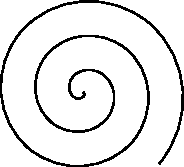
\includegraphics[width=8cm]{pics/spiral.pdf}
\caption{A spiral... smooth vector-based with a clean parametrisation! \\ Nothing to do with \cite{Gage:18}}\label{fig:spiral}
\end{figure}
\FloatBarrier

\section{Tables}

\begin{table}[H]
\small
\centering
\begin{tabular}{p{5cm}|l|p{3cm}}
`` Industrial era '' &  ``Jobs '' & `` Wanted: Upgrade''' \\ \hline
Parts exchanger & Fitter & mecatronics specialist \\
eShop & reseller & `` Client-suggester'' \\
`` Coding-guru''' & Softwaredesign & Whole-life designer \\
JA! Gut \& Günstig & brand-names & `` Life-Style Feeling'' \\
Internetbanking & Bank clerk & Customer adviser \\
Robots & Specialist & Machine supervisor \\
Bush & Gardener & Nature-sculptor \\
Painting & Painter & Interior Design \\
 &  & \\
\end{tabular}
\caption[Downgrade and upgrade of job denominations]{Downgrade and Upgrade of job denominations \\ \ \ \ \cite{DueckKo:2016}}
\label{tab:Downgrade and Upgrade of job denominations}
\end{table} 

\section{Listes}

\begin{itemize}
 \itemsep0pt
 \item one
 \item twoi
 \item threei
\end{itemize}

\begin{enumerate}
 \itemsep0pt
 \item first
 \item second
 \item third
\end{enumerate}


\section{Formulæ}

A formula can be written inline, e.g. as $ \frac{d}{dx}\mbox{arctg}(x) = \frac{1}{1+x^2}$ or, in centered math:

\begin{equation}  \frac{d}{dx}\mbox{arctg}(x) = \frac{1}{1+x^2} \label{arctanderivative}\end{equation}

Notice that formulæ that are centered start bigger (technically, they start in \verb+\displaystyle+) than they start inline (technically, they start in \verb+\textstyle+ all subsequents reductions, e.g. an exponent, goes to \verb+\scriptstyle+ then \verb+\scriptscriptstyle+). Indeed a best effort is made so that inline formulæ do not change the line height which would bother the eye of a reader.

Formulæ can be given a number and a label. Numbering happens automatically with \verb+\begin{equation}+ and \verb+\end{equation}+ and can be avoided if enclosing the formula betwee \verb+\[+ and \verb+\]+. If using the \verb+\label+ macro inside, you can refer automatically to this equation using \verb+\ref{label}+. E.g. Thanks to equation~\ref{arctanderivative} one dare say that:

\begin{equation} \int_0^t \frac{1}{1+x^2} dx = \mbox{arctan}(t) \end{equation}
%\chapter{Conclusion}


\appendix 

% ---- Bibliography ----
%
% BibTeX users should specify bibliography style 
% References will then be sorted and formatted in the correct style.
%
 %\bibliographystyle{alpha}
\bibliographystyle{iubh}
\bibliography{biblio}

%\printbibliography[heading=none]

%\chapter{Annexes (optional)}

(with a list of them)



%\chapter{Glossary (optional)}

\chapter*{Eidesstattliche Erklärung}

\begin{figure}[t!]
    \raggedleft
    
\includegraphics[scale=0.3]{pics/logo.pdf}
\end{figure}

\thispagestyle{empty} %Seitenzahl weglassen

I hereby certify...


\vspace{1,5 cm} 
\begin{tabular}{p{7cm}p{.5cm}l}
\dotfill \\ 
Place, date
\end{tabular}% 
\hfill 
\begin{tabular}{p{7cm}p{.5cm}l}
\dotfill \\ 
Signature
\end{tabular}% 

\end{document}
